% Number 910
% CAPMA Algebra  Units 
% US Open putt
% JG

% Watermark
\AddToShipoutPicture*{\BackgroundPic}

\addtocounter {ProbNum} {1}

%\begin{floatingfigure}[r]{.44\textwidth}
%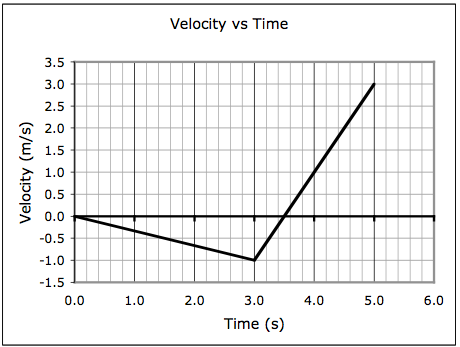
\includegraphics[scale=.54]{/Users/jgates/desktop/latex/pics/vgraph6}
%\end{floatingfigure}
 
{\bf \Large{\arabic{ProbNum}}} In the US Open, you need to make a 7.2 meter putt to win.  You give the ball an initial speed of 4.6 meters per second, but it stops 1.8 meters short of the hole.  (That's OK: you still get a really big check!) \bigskip

If you had hit the ball with the minimum initial speed that would have gotten it into the hole, how long would you have had to wait breathlessly to see if it was going to roll in?
\vfill


%\begin{center}
%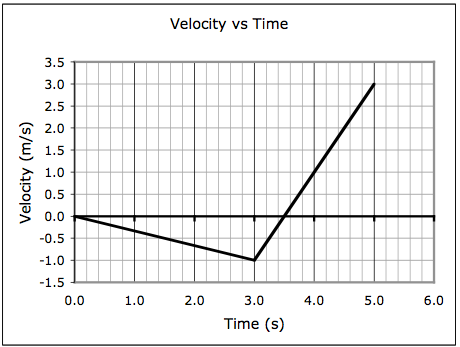
\includegraphics[scale=1]{/Users/jgates/desktop/latex/pics/vgraph6}
%\end{center}


\newpage